\documentclass{csmathnotes}

\udc{004.912}
\title{Задача извлечения именованных сущностей в русскоязычном тексте}

\author{Аверина Мария Дмитриевна}
\position{магистр}
\affiliation{Ярославский государственный университет им. П.\,Г. Демидова}
\email{maverina518@gmail.com}

\author{Дунаева Ольга Александровна}
\position{к.ф.-м.н.}
\affiliation{Ярославский государственный университет им. П.\,Г. Демидова}
\email{olaydy@gmail.com}

\usepackage{diagbox}
\addbibresource{Averina.bib}


\begin{document}

\maketitle

\begin{abstract}
В статье рассматривается задача извлечения именованных сущностей из текста.
Для решения данной задачи часто используется метод \emph{CRF} "--- условные случайные поля.
В статье исследуется вопрос решения задачи извлечения именованных сущностей для текста на русском языке на основе метода условных случайных полей.
При этом были использованы различные подходы к признаковому описанию текста,
был проведен сравнительный анализ моделей при использовании различных признаков и методов оптимизации.
Лучшая модель показала качество \emph{F1} равное $75\,\% - 99\,\%$ в зависимости от сущности.
\end{abstract}

\keywords{распознавание именованных сущностей, \emph{NER}, условные случайные поля, \emph{CRF}, токенизация, нормализация слов, \emph{word2vec}, \emph{fastText}, \emph{F1}}.

\section*{Введение}
Одна из важнейших задач – сбор и анализ статистических данных нормативных
документов является достаточно трудоемкой для специалистов. На данный момент, в условиях повсеместного внедрения электронного документооборота, данная задача особенно актуальна. Автоматизация процесса анализа текстов – задача распознавания именованных сущностей~(named entity recognition, \emph{NER})~\cite{base} позволит оптимизировать работу многих специалистов как по временным, так и по качественным показателям.


\section*{Задача извлечения сущностей}

Задача NER заключается в выделении определенных непрерывных фрагментов текста~(именованных сущностей).
Например, имеется новостной текст, в котором необходимо выделить некоторый заранее зафиксированный набор сущностей: персоны, локации, организации, даты и т.д.
Соответственно алгоритм должен определить, что участок текста «1 января 1997 года» является датой, «Кофи Аннан» – персоной, а «ООН» – организацией~(рис.\ref{fig:ner}).


\begin{figure}[h]
    \center{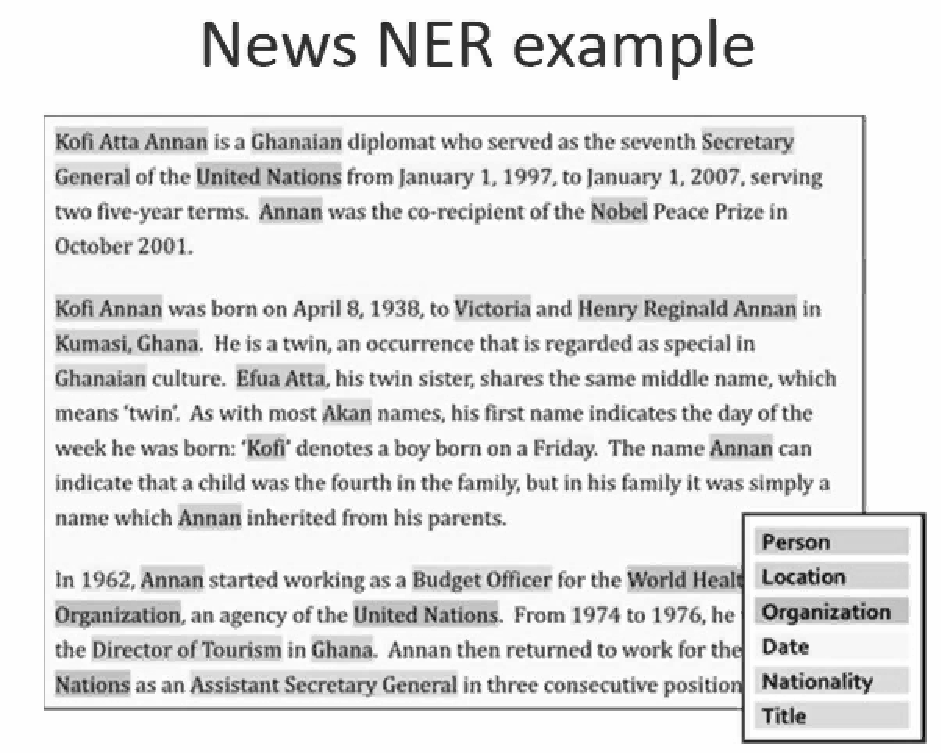
\includegraphics[scale=0.5]{1.pdf}}
    \caption{Пример работы NER.}
    \label{fig:ner}
\end{figure}


Данная статья посвящена задаче выделения именованных сущностей для рускоязычных текстов.
В качестве тестовых данных была использована открытая база судебной статистики~\cite{CourtsData}.
Такой выбор был сделан в силу большого количества доступных документов, а также соответствующего задаче характера текстов~(наличие множества различных имён, дат, наименований, сумм и т.д.)

На основе данной базы была сформирована и размеччена выборка из $500$ файлов, которая была размечена на инструменте BRAT. BRAT (brat rapid annotation tool) — онлайн-инструмент для разметки письменных текстов. Были выделены следующие сущности: номер документа (doc num), суд (court), судья (judge), дата суда (date court), истец (plaintiff), ответчик или представитель (defendant), решение суда (court decision), статья или тип штрафа (payment fine), сумма выплаты (payment amount), срок обжалования (appeal time).


\section*{Предварительная обработка данных}
Первым этапом решения задачи является предобработка данных, которая включает в себя разбиение текста на слова, удаление ненужных символов, и извлечение признаков слов. 
Токенизация — это процесс разбиения текстового документа на отдельные слова, которые называются токенами.
Для начала весь текст был разбит на токены~\cite{ner}, при этом удалены символы, не несущие смысловой нагрузки, и слова приведены к нижнему регистру.


Одним из наиболее очевидных признаков для решения задачи классификации именованных сущностей является вычленение информации при помощи регулярных выражений. Например, информация о наличие заглавной буквы или знаков препинания после слова заносится в  «словарь символов». «Словарь символов» "--- структура данных, которая хранит в себе информацию о находящихся рядом знаках препинания и о регистре букв слова.
Например почта \emph{<<v1@mail.com,>>} будет разбита на \emph{<<v1@>>} и \emph{<<mail.com,>>}, где @ идентифицируется как слово-спецсимвол, а запятая заносится в «словарь символов». Символ @, позволяет классифицировать строку как почтовый адрес. Используемые нами спецсимволы: @, \#, №,\,\%, $/$.


Приведем список признаков в «словаре символов»:
\begin{itemize}
    \item первая буква большая, остальные маленькие;
    \item все буквы маленькие;
    \item все буквы большие;
    \item первая буква маленькая;
    \item наличие запятой или точки в конце или начале слова и т.д.
\end{itemize}


Также в качестве признака можно использовать <<само слово>>. Стоит отметить, что данный признак не является релевантным, если в обучающей выборке часто упоминается одна и та же фамилия или одно и тоже название организации, поскольку алгоритм «зацепляется» за конкретное слово.
Например для тестов судов, фамилия судьи встречается в тексте несколько раз.


Большинство слов в тексте имеет падеж или склонение, что в свою очередь усложняет работу алгоритма.
Одним из способов решения данной проблемы является нормализация слов "--- приведение их к стандартному виду
(например, лосями $\rightarrow$  лось, мыла $\rightarrow$ мыть, зеленого $\rightarrow$ зеленый).
При этом число и род можно использовать как признаки.
Также часть речи (существительное, предлог и т.д.), является неплохим признаком при распознавании сущностей.
Отметим, что в случае слов-спецсимволов, можно каждому символу задать уникальные значения частей речи.
Например, для символа \,\% морфологией будет \emph{PERCENT}.

 
Другим распространенным подходом к вычислению признаков является векторизация слов "---  представление слова в виде вектора~\cite{w2v}.
После предобработки текста слова можно закодировать векторами чисел, которые в дальнейшем удобно использоваться при обучении.
Алгоритм \emph{Word2Vec} работает с большими текстовыми данными и по определенным правилам присваивает каждому слову уникальный набор чисел "--- семантический вектор. Спустя некоторое время появились улучшения данного алгоритма, например  из модификаций часто используемым является \emph{fastText}. FastText исправляет недостаток метода Word2Vec: если обучение модели начинается с прямого кодирования одного D-мерного вектора, то игнорируется внутренняя структура слов. Вместо прямого кодирования слов, алгоритм fastText предлагает изучать N-граммы символов и представлять слова как сумму векторов N-грамм.


Для улучшения качетсва обучения, можно учитывать не только признаки текущего токена, но и соседних токенов, тем самым учитывая контекст.
В дальнейшем для используемых признаков будем использовать обозначения: <<список символов>> "--- \emph{r}, <<само слово>> "--- \emph{v}, часть речи "--- \emph{m}, нормализация "--- \emph{n}, Word2Vec "--- \emph{w}, FastText "--- \emph{f}.
А цифра после буквы будет обозначать количество рассматриваемых соседей влево и вправо.
Например, \emph{f3} означает, что использовалось $7$ признаков FastText "--- для текущего слова и для 3-х соседей с каждой стороны.

\section*{Прогнозирование тегов при помощи CRF}
Наиболее  популярный инструмент для решения задачи распознавания именованных сущностней является метод CRF (conditional random fields, условные случайные поля)~\cite{HabrCRF}. 
Алгоритм оптимизирует всю цепочку меток целиком, а не каждый элемент по отдельности, учитывает любые особенности и взаимозависимости в исходных данных, а также он хорошо работает в связке с рекуррентными нейросетями, моделирует совместное распределение на всей последовательности выходов сети одновременно.

Линейный CRF хорошо подходит для решения задач сегментации и разметки последовательности,
например: автоматическое выделение ключевых слов из текстов, выделение именованных сущностей (классификация сущностей), анализ тональности, автоматическое распознавание речи.


Процесс обучения имеет большую вычислительную сложность, а именно $O(mNTQ2nS)$ где:
\begin{itemize}
    \item \emph{m} — количество тренировочных итераций;
    \item \emph{N} — количество обучающих последовательностей;
    \item \emph{T} — средняя длина обучающей последовательност;
    \item \emph{Q} — количество выходных классов;
    \item \emph{n} – количество признаков в обучающей матрице;
    \item \emph{S} – время работы алгоритма оптимизации на каждом шаге. 
\end{itemize}


На практике время обучения даже выше за счет всевозможных дополнительных операций таких, как сглаживание, преобразование данных из одного формата в другой.
Отметим, что при увеличении количества признаков, например, за счет соседних слов, время обучения значительно увеличивается. 

\section*{Метрика F1}
После того как CRF обучен необходимо оценить качество его работы. Метрики точности (Precision, P) и полноты (Recall, R) дают исчерпывающую оценку качества, но, как правило, приходится балансировать между двумя этими метриками.
Если повысить полноту, делая решение более «оптимистичным», это приводит к падению точности из-за увеличения числа ложно-положительных ответов.
Если же наоборот, то при росте точности происходит одновременное падение полноты из-за отбраковки какого-то числа правильных ответов.
Поэтому удобно использовать одну величину, так называемую метрику \emph{F1} "--- среднегармоническое между полнотой и точностью:

\begin{equation}
F1 = 2\frac{P\times R}{P + R} 
\end{equation}

Для оценки качества полученных результатов было решено использовать F1, но полноту и точность вычислять, путем объединения соседних слов с одним тегом в одну сущность.
Поскольку одна сущность может состоять из нескольких токенов, то стоит при оценке качества учитывать ее целиком. 

\section*{Результаты}
Обучение проводилось на $400$ файлах данных судебных протоколов, а также для тестирования была отложена выборка из $100$ документов. Наилучшего качества можно добиться за счет подбора параметров метода CRF. В данной работе были протестированы алгоритмы оптимизации CRF. В таблице~\ref{tabl:table1} приведен анализ оптимизаторов, при одном фиксированном наборе признаков. 

\begin{itemize}
    \item \emph{lbfgs} "--- градиентный спуск с использованием метода 
    \emph{L-BFGS};
    \item \emph{l2sgd} "--- стохастический  градиентный спуск \newline с регуляризацей \emph{L2};
    \item \emph{pa} "--- усредненный персептрон;
    \item \emph{ap} "--- passive аggressive;
    \item \emph{arow}"--- адаптивная регуляризация.
\end{itemize}

\begin{table}[!h]
    \begin{center}
        \begin{tabular}{|p{2cm}|p{1.6cm}|p{1.5cm}|p{1.5cm}|p{2.5cm}|}
            \hline
            Алгоритм оптимизации &  Долгое время работы & \emph{F1} на лучшей сущности & \emph{F1} на худшей сущности & Примечания \\
            \hline
            \emph{lbfgs} & $+$ & $1$ & $0.7$ & Время обучения более $5$ часов.  \\
            \hline
            \emph{l2sgd} & $+$ & $1$  & $0$ & Классифицирует все, как самый. объемный класс \\
            \hline
            \emph{pa} & $-$ & $1$  & $0.45$ & Время обучения не более $30$ минут. \\
            \hline
            \emph{ap} & $-$ & $0.83$ & $0.24$  & $-$ \\
            \hline
            \emph{arow} & $-$ & $0.79$ & $0.31$  & $-$ \\
            \hline
        \end{tabular}
    \end{center}
    \caption{\label{tabl:table1}Сравнительный работы CRF при использовании различных оптимизаторов.}
\end{table}

Как видно из таблицы~\ref{tabl:table1} лучший результат показали алгоритмы оптимизации \emph{pa} и \emph{lbfgs}. Стоит отметить, что \emph{lbfgs}  более трудоемкий по сравнению с \emph{pa}. В дальнейших тестах для выбора оптимальных признаков были использованы данные два оптимизатора.


После выбора оптимизаторов, было проведено тестирования на различных признаках. В таблице~\ref{tabl:table2} приведены результаты данного тестирования, где сверху вниз в ячейках указаны F1 на лучшей сущности, F1 на худшей сущности, время обучения модели. Заметим, что наименьший разброс F1  принимает при $(r3,v3)$ с оптимизатором \emph{lbfgs}, при этом демонстрируя достаточно высокий средний результат. Однако, время обучения такой модели более пяти часов. При необходимости уменьшить время обучения наиболее оптимальным решением будет обучение модели на признаках $(r3,v1)$ с оптимизатором \emph{pa}.

\begin{table}[h]
	\begin{center}
		\begin{tabular}{|p{2.1cm}|p{2.5cm}|p{2.5cm}|p{2.5cm}|}
			\hline
			\diagbox[width=7.2em]{Признаки}{Алгоритм} &  \emph{pa} & \emph{l2sgd} & \emph{lbfgs} \\
			\hline
			$(r3, v3)$ & $-$ & $-$ & 
			doc num  $0.993$ \newline
			defendant  $0.751$ 
			\newline  $5.55.36$ \\
			\hline
			$(r3, v1)$ & judge $0.906$ \newline
			defendant   $0.455$ 
			\newline $0.07.58$
			& judge  $0.867$ \newline
			defendant    $0.116$ \newline
			$0.4.11$
			& doc num  $0.973$ \newline
			defendant  $0.685$\newline
			$3.32.49$ \\
			\hline
			$(w1, v1, m1)$ 
			& court   $0.827$ \newline
			defendant   $0.331$ \newline
			$0.05.20$
			& judge    $0.751$ \newline
			court  $0.013$ \newline
			$0.3.14$
			& judge $0.971$\newline
			defendant  $0.541$\newline
			$3.03.01$\\
			\hline
			$(r3, m3)$
			& judge $0.692$ \newline
			payment $0.412$ \newline
			$0.33.58$
			& date court   $0.746$ \newline
			court $0.126$ \newline
			$0.12.11$
			& judge $0.818$ \newline
			defendant $0.285$ \newline 
			$3.58.24$\\
			\hline
		\end{tabular}
	\end{center}
	\caption{\label{tabl:table2}Сравнительный анализ F1 на различных наборах признаков.}
\end{table}

\section*{Заключение}
В статье рассмотрен подход к решению задачи извлечения именованных сущностей. При решении поставленной задачи был использован метод CRF. В работе были представлены наборы различных текстовых признаков для CRF. 
Затем был проведен сравнительный анализ алгоритмов оптимизации и признаков, который показал, что алгоритм \emph{pa} с признаками $(r3, v1)$ показал наилучший результат по времени и F1 в совокупности. Алгоритм оптимизации \emph{lbfgs}  с признаками $(r3, v3)$ продемонстрировал лучший результат по F1, но оказался трудоемким и долгообучаемым. Стоит отметить, что лучший результат  по времени показал алгоритм \emph{pa}. Однако, для более точного прогнозирования лучшим подходом является использование алгоритма оптимизации \emph{lbfgs}.


Для дальнейшего улучшения результатов планируется извлекать дополнительные признаки. Также перспективным направлением разработки является исследование альтернативных методов классификации на основе biLSTM и BERT.

\printbibliography

\end{document}
